%% Temperature-Parametrised Kalman Priors and Learned Corrections for Li-ion SOC Estimation
%% IEEE Transactions style (IEEEtran), pdfLaTeX. All numbers are generated from the MATLAB result files.
\documentclass[journal]{IEEEtran}

\usepackage[T1]{fontenc}
\usepackage{amsmath,amssymb}
\usepackage{graphicx}
\usepackage{booktabs}
\usepackage{array}
\usepackage{xcolor}
\usepackage{cite}
\usepackage{url}
\usepackage{microtype}
\usepackage[hidelinks,breaklinks]{hyperref}

% numbers are inserted by the generator from the MATLAB result files

%% ---- notation ----
\newcommand{\T}{^{\!\top}}
\newcommand{\SOC}{\mathrm{SOC}}
\newcommand{\OCV}{\mathrm{OCV}}
\newcommand{\vx}{\boldsymbol{x}}
\newcommand{\vw}{\boldsymbol{w}}
\newcommand{\mP}{\mathbf{P}}
\newcommand{\mH}{\mathbf{H}}
\newcommand{\mK}{\mathbf{K}}
\newcommand{\mQ}{\mathbf{Q}_{\mathrm{w}}}
\newcommand{\pend}[1]{\textcolor{red}{[pending rerun: #1]}}
\newcommand{\mA}{\mathbf{A}}
\newcommand{\mB}{\mathbf{B}}
\newcommand{\mI}{\mathbf{I}}

\emergencystretch=1.5em
\hyphenpenalty=750


\begin{document}

\title{Temperature-Parametrised Kalman Priors and Learned Corrections for Lithium-Ion State-of-Charge Estimation Across Temperatures and Cells}

\author{Suyash~D.~Nahar,~Keya~Bist,~Isha~Priya,~and~Dastagiri~B.~Reddy\\
\normalsize Department of Electrical and Electronics Engineering, National Institute of Technology Karnataka (NITK),\\
\normalsize Surathkal, Mangaluru, Karnataka~575025, India%
\thanks{Manuscript received XX XX, 2026. Corresponding author: S.~D.~Nahar.}}

\markboth{IEEE Transactions, Vol.~XX, No.~X, 2026}{Nahar \MakeLowercase{\textit{et al.}}: Temperature-Parametrised Kalman Priors and Learned Corrections for SOC Estimation}

\maketitle


\begin{abstract}
A state-of-charge (SOC) estimator for electric vehicles has to work at temperatures, on drive cycles, and on cells that were not in its training data. We test one design on that requirement: four Kalman filters on a first-order Thevenin circuit whose parameters at unmeasured temperatures follow an Arrhenius law, three learners (a bidirectional LSTM, a physics-informed LSTM, and boosted trees) that predict a correction to a Kalman prior, and a simplex-constrained stacking layer. Eleven protocols on three public datasets separate unseen drive cycles, a held-out temperature, extrapolation to colder temperatures, sparse calibration, and transfer to a second cell, and every estimator starts from a 10--20\% initial SOC error. The bidirectional LSTM lowers the error of the best filter from 3.71\% to 1.57\% RMSE on unseen cycles of the LG cell and from 6.70\% to 2.24\% on the Samsung cell, and the Arrhenius circuit model lowers the best-filter error from 4.36\% to 2.04\% at a held-out temperature and from 10.58\% to 6.05\% in extrapolation. The design has clear limits. Stacking is never the most accurate estimator and the physics term brings no benefit that five seeds separate from noise. A raw-input network, most often the LSTM fused with Coulomb counting, is more accurate than all of our estimators on four of the ten protocols where it was run (S-L, S-X, S-E, B-W; on S-X it uses target-cell training) and is level with them on LG-T. At $-20$~$^\circ$C without training data there, the best estimate is 10.30\% RMSE on the LG cell and 13.36\% on the Samsung cell, and identifying the circuit parameters directly does not remove the error. On a held-out drive cycle the best filter (4.95\%) beats every learner (6.44\% or worse).
\end{abstract}

\begin{IEEEkeywords}
Battery management systems, Kalman filtering, long short-term memory, residual learning, state-of-charge estimation, temperature generalisation.
\end{IEEEkeywords}

\section{Introduction}
\IEEEPARstart{S}{tate} of charge (SOC), the charge available in a cell relative to its capacity, governs range prediction, charge and discharge limits, and ageing management in a battery-electric vehicle~\cite{xiong2018review,plett2015bms}. SOC cannot be measured. It is reconstructed from terminal voltage, current, and temperature, which carry noise, offsets, and parameter drift. Recursive observers compare the measured voltage with the voltage predicted by an equivalent-circuit model and feed the difference back into the state~\cite{plett2004ekf,chen2013ekf}; recurrent networks learn the map from the measurements to SOC directly~\cite{chemali2017lstm}.

\textbf{The problem.} A deployed estimator meets conditions its designers did not measure: a temperature between or beyond the calibrated ones, a drive cycle that is not in the training set, a cell of another type, and a start-up SOC that is wrong. Observers degrade in the cold, where resistance and polarisation change strongly~\cite{xiong2018review,hannan2017review}, and where parameters identified per temperature are unavailable for temperatures that were never measured. Networks trained on raw signals depend on how much of the operating range the training data cover~\cite{zhao2024wevj,hu2026ionics}. Much of the hybrid literature reports one cell and one split, so generalisation across cycles, temperatures, and cells is rarely quantified.

\textbf{What we do.} Four Kalman filters on a first-order Thevenin model supply SOC priors. Where a temperature has no identification data, the circuit parameters follow an Arrhenius law fitted to the identified temperatures. Three learners predict the correction to one Kalman prior rather than SOC itself, and a non-negative stacking layer on the probability simplex merges the seven estimates. One global model serves all temperatures, with temperature as an input. Eleven protocols (Table~\ref{tab:protocols}) separate interpolation, held-out temperature, extrapolation, sparse calibration, and cross-cell transfer, and four raw-input reference models, including an LSTM fused with Coulomb counting in a Kalman filter, are evaluated on the same splits.

\textbf{What we find.}
(i)~On unseen drive cycles the bidirectional LSTM reduces the error of the best filter by 58\% on the LG cell and by 67\% on the Samsung cell, and at least one learner beats the best filter in ten of eleven protocols.
(ii)~The Arrhenius circuit model lowers the best-filter error by 53\% at a held-out temperature and by 43\% in extrapolation, but not under sparse calibration.
(iii)~Outside the training temperature range the Kalman prior bounds the error of the LG learners (6.06--6.18\%) where raw-input models reach 12.09--19.62\%; on the Samsung cell the same raw-input models are close (7.29--12.42\% against 8.50\%), so the protection is not general.
The same experiments show where the design does not win: stacking is not the best estimator in any protocol, the Coulomb-counting loss does not help, a raw-input LSTM with Coulomb counting is competitive in range, the filters beat the learners on a held-out drive cycle, and nothing is accurate at $-20$~$^\circ$C without training data there.

\textbf{Contributions.}
\begin{enumerate}
\item A temperature-parametrised circuit model for the filter priors (Arrhenius for $R_0$, $R_1$, $\tau_1$ and a low-order law for capacity), evaluated against a nearest-temperature lookup on six temperature protocols, with a parameter-oracle experiment that locates what the extrapolation gets wrong.
\item Residual learning on filter priors with a prior chosen by a validation rule, quantified in range, out of range, across cells, and on a held-out cycle.
\item An evaluation with its negative results in one place (Section~\ref{sec:neg}): five-seed statistics, segment-level intervals, Coulomb-counting baselines, convergence times, robustness, and a measured latency on an embedded Linux board (Arduino UNO Q).
\end{enumerate}
Section~\ref{sec:related} places the work against the literature, Sections~\ref{sec:overview}--\ref{sec:fusion} describe the method, Section~\ref{sec:setup} the protocols, and Section~\ref{sec:results} the evidence.

\section{Related Work}\label{sec:related}
\subsection{Reviews}
Surveys classify SOC estimation into Coulomb counting, OCV lookup, model-based observers, data-driven models, and hybrids~\cite{xiong2018review,hannan2017review}. Recent reviews organise the field around machine learning~\cite{zhao2024wevj} and around accuracy, robustness to temperature and ageing, computational cost, and on-board feasibility, and they name physics-informed learning, cross-condition generalisation, and edge deployment as open directions~\cite{hu2026ionics}. A review of machine-learning state-of-health estimation concludes similarly that hybrid data-model approaches are the route to robust generalisation~\cite{wang2025rser}. This paper answers those directions with measured cross-temperature, cross-cell, and latency results, including the cases where the proposed combination does not win.

\subsection{Circuit Models, Temperature, and Data-Driven Estimators}
Equivalent-circuit models of low order are the usual basis of on-board observers~\cite{hu2012ecm,plett2015bms}, and their parameters depend strongly on temperature, mainly through a thermally activated rise of the resistances in the cold~\cite{jaguemont2016cold,waag2014review}. Studies that identify the circuit separately at each temperature need data at every temperature of use; here the Arrhenius form is fitted to the measured temperatures and extended to others, and its limits are measured. On the learning side, recurrent networks and their bidirectional variants estimate SOC from the raw measurements~\cite{chemali2017lstm,bian2020bilstm,hochreiter1997lstm,schuster1997birnn}, feedforward networks have been trained on the same LG data over a range of temperatures~\cite{vidal2020ffnn}, and transfer learning is used to adapt a network to a new temperature or cell~\cite{vidal2019transfer,pan2010transfer}. Physics-informed training adds a residual of a known law to the loss~\cite{raissi2019pinn}; here the law is Coulomb counting, and its effect is tested against a variant without it.

\subsection{Hybrid Filter and Learning Methods}
Hybrids combine a learned model and a filter in several ways: the filter smooths a network output~\cite{xu2025processes,jiang2025energy}, a network supplies a pseudo-measurement to a filter~\cite{previtali2025iecon}, or a Coulomb-counting term enters the loss~\cite{pollo2025date}; weighted combinations of Coulomb counting and a recurrent network have also been reported~\cite{carrera2025sensors}. Here the filters are priors for the learners, four filter mechanisms are compared on one model, and the final merge is a label-free convex layer over seven estimators. Because the pseudo-measurement approach is the closest to this work, a version of it (an LSTM on the raw inputs fused with Coulomb counting in a scalar Kalman filter, called LSTM+KF) is implemented and evaluated on ten of the eleven splits. Table~\ref{tab:related} lists representative studies; their errors are on different data and splits and are not directly comparable with those in Section~\ref{sec:results}. Stacked generalisation is established in machine learning~\cite{wolpert1992stacked,breiman1996stacked}; to the authors' knowledge, its combination with filter priors for SOC has not been reported in the studies surveyed here.

\begin{table}[!t]
\caption{Representative Hybrid SOC Studies (Reported Values, Different Data; Not Directly Comparable)}
\label{tab:related}
\centering
\footnotesize
\setlength{\tabcolsep}{3pt}
\begin{tabular}{p{1.1cm}p{3.0cm}p{2.1cm}p{1.6cm}}
\toprule
Work & Hybridisation & Data & Reported error\\
\midrule
\cite{xu2025processes} & CNN-LSTM, adaptive KF smoothing & LG HG2, DST/FUDS/US06 & RMSE $<1.51\%$\\
\cite{jiang2025energy} & PatchMixer-LSTM, adaptive UKF & US06, FUDS & RMSE 0.12\% (50~$^\circ$C)\\
\cite{pollo2025date} & Coulomb-counting loss, two-branch network & Sandia, LG HG2 & MAE 0.014 (LG, 25~$^\circ$C)\\
\cite{previtali2025iecon} & Learned virtual sensor fused in EKF & Samsung 21700 & RMSE 1.9\%\\
\cite{carrera2025sensors} & Coulomb counting and GA-tuned LSTM & LiFePO$_4$ packs & RMSE 0.48\%\\
This work & Arrhenius-parametrised filter priors, residual learners, simplex stacking & LG HG2, Samsung 30T, six temperatures, unseen cycles & RMSE 1.57\% (LG), 2.24\% (Samsung), BiLSTM\\
\bottomrule
\end{tabular}
\end{table}

\section{Framework}\label{sec:overview}
Fig.~\ref{fig:arch} shows the data flow. The measured signals $V$, $I$, and $T$ enter four Kalman filters that run on a first-order Thevenin model whose parameters are identified, or extended by the Arrhenius law, for the temperature of the segment. Their SOC estimates, concatenated with the measured and derived signals, form the feature vector. The PI-LSTM receives all 11 features, and the BiLSTM and LSBoost receive an 8-feature subset that carries the EKF prior and the prior to be corrected (SPKF or SHEKF, whichever has the lower validation RMSE of the fused estimate; Section~\ref{sec:tuning}). Each learner predicts the correction to that prior, and the seven estimates (four filters, three learners) enter the stacking layer, which returns the fused SOC.

\begin{figure*}[!t]
\centering
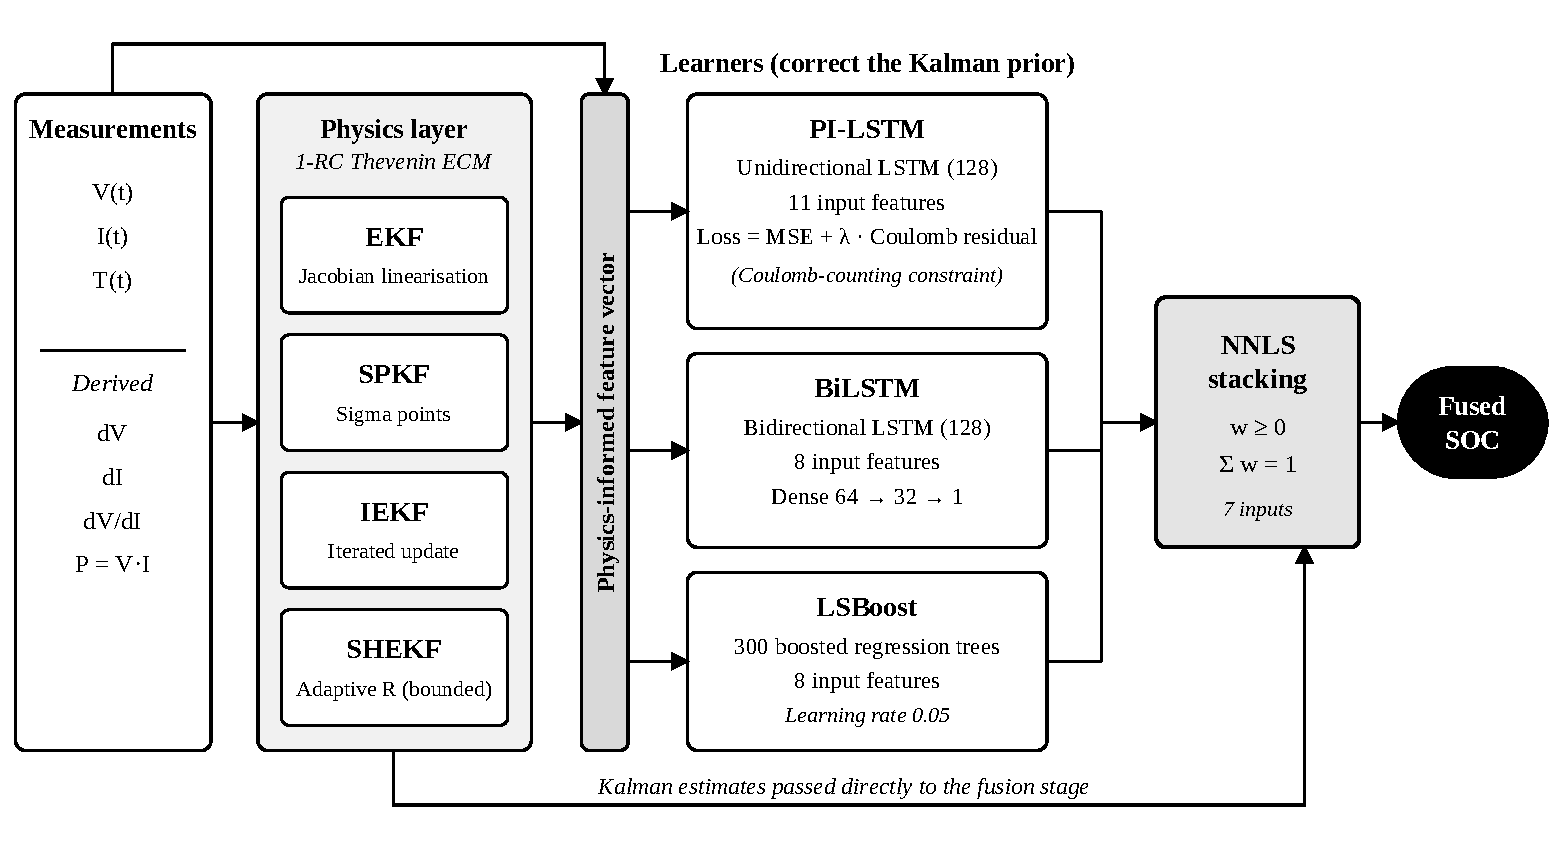
\includegraphics[width=0.97\textwidth]{figs/soc_architecture_final.pdf}
\caption{Framework. Four Kalman filters on a 1-RC model with temperature-parametrised parameters generate SOC priors; the learners predict the correction to one Kalman prior; the simplex stacking layer combines the seven estimates.}
\label{fig:arch}
\end{figure*}

\section{Equivalent Circuit Model}\label{sec:ecm}
A first-order Thevenin circuit has an OCV source, an ohmic resistance $R_0$, and one polarisation branch $(R_1,C_1)$. With state $\vx_k=[\SOC_k,\,V_{RC,k}]\T$ and sampling interval $\Delta t=1$~s,
\begin{align}
\vx_{k+1} &= \mA\vx_k+\mB I_k+\mathbf{w}_k,\\
V_k &= \OCV(\SOC_k)-V_{RC,k}-R_0 I_k+v_k,
\end{align}
with
\begin{equation}
\mA=\begin{bmatrix}1&0\\0&\alpha\end{bmatrix},\quad
\mB=\begin{bmatrix}-\Delta t/Q_{\mathrm{cap}}\\ R_1(1-\alpha)\end{bmatrix},\quad \alpha=e^{-\Delta t/\tau_1},
\end{equation}
$\tau_1=R_1C_1$, $Q_{\mathrm{cap}}$ the capacity in ampere-seconds, and $\mathbf{w}_k\sim\mathcal N(\mathbf 0,\mQ)$ the process noise. Discharge current is positive. For the two Kollmeyer cells the parameters are identified separately at each chamber temperature that the protocol makes available. The OCV curve is the mean of the C/20 discharge and charge curves at that temperature. $(R_0,R_1,\tau_1)$ are fitted to the fit-block drive data by multi-start least squares (eight starts) on the voltage prediction error with $\tau_1$ bounded to $[1,600]$~s, and $Q_{\mathrm{cap}}$ is the temperature-specific discharged charge. Table~\ref{tab:ecm} gives the identified values for the LG cell. $R_0$ rises by a factor of about 5 from $+25$ to $-20$~$^\circ$C. All eight starts converge to the same point at every temperature, so local minima do not explain the values. The identified $R_1$ is nearly equal at $-10$ and $-20$~$^\circ$C (64.54 and 64.50~m$\Omega$, all eight starts agreeing at each temperature, so a flat optimum of the voltage fit and not a bound) while $\tau_1$ falls from 41.7 to 19.1~s; this suggests that the one-branch model absorbs cold-temperature behaviour (hysteresis, diffusion) that it cannot represent, and it limits the physical reading of the individual parameters. For the Braun record a single parameter set is identified because the cell is held near constant temperature.

\begin{table}[!t]
\caption{Identified 1-RC Parameters, LG 18650HG2 (Unseen-Cycle Run)}
\label{tab:ecm}
\centering\small
\begin{tabular}{rcccc}
\toprule
$T$ ($^\circ$C) & $R_0$ (m$\Omega$) & $R_1$ (m$\Omega$) & $\tau_1$ (s) & $Q_{\mathrm{cap}}$ (Ah)\\
\midrule
$-20$ & 95.3 & 64.5 & 19.1 & 1.617 \\
$-10$ & 58.0 & 64.5 & 41.7 & 2.232 \\
$0$ & 39.8 & 48.5 & 52.8 & 2.450 \\
$10$ & 29.2 & 37.2 & 54.9 & 2.485 \\
$25$ & 20.3 & 18.1 & 25.6 & 2.693 \\
$40$ & 17.9 & 15.3 & 23.9 & 2.658 \\
\bottomrule

\end{tabular}
\end{table}

\subsection{Parameters at Temperatures Without Identification Data}\label{sec:arrh}
Let $T$ be the cell temperature in kelvin and $\mathcal T_{\mathrm{id}}$ the identified temperatures. For a temperature outside $\mathcal T_{\mathrm{id}}$, each of $\ln R_0$, $\ln R_1$, $\ln\tau_1$, and $\ln R_n$ is a linear function of $1/T$ fitted by least squares over $\mathcal T_{\mathrm{id}}$, the Arrhenius form $R=R_{\mathrm{ref}}\exp\{E_a/k\,(1/T-1/T_{\mathrm{ref}})\}$ of a thermally activated process. The capacity is a linear function of $T$ (quadratic when at least four temperatures are available), the OCV curve of the nearest identified temperature is used, and time constants are clipped to $[1,600]$~s. Table~\ref{tab:arrh} compares the values predicted from identification at $\ge10$~$^\circ$C with direct identification. At $0$~$^\circ$C the model is within 15\% for $R_0$ and within 1\% for $R_1$ and the capacity. At $-20$~$^\circ$C it underestimates $R_0$ by 45\%, overestimates $R_1$ by 61\%, $\tau_1$ sevenfold, and the capacity by 46\%. Section~\ref{sec:temp} tests how much of the extrapolation error this causes (it explains part of the error at $0$ and $-10$~$^\circ$C, and not the error at $-20$~$^\circ$C).

\begin{table}[!t]
\caption{LG: Arrhenius Prediction From $\ge10$~$^\circ$C / Direct Identification}
\label{tab:arrh}
\centering\footnotesize
\setlength{\tabcolsep}{3pt}
\begin{tabular}{rcccc}
\toprule
$T$ ($^\circ$C) & $R_0$ (m$\Omega$) & $R_1$ (m$\Omega$) & $\tau_1$ (s) & $Q_{\mathrm{cap}}$ (Ah)\\
\midrule
$0$ & 34.1 / 39.8 & 48.4 / 48.5 & 68.3 / 52.8 & 2.468 / 2.450 \\
$-10$ & 41.7 / 58.0 & 69.9 / 64.5 & 96.6 / 41.7 & 2.410 / 2.232 \\
$-20$ & 52.0 / 95.3 & 103.9 / 64.5 & 140.4 / 19.1 & 2.353 / 1.617 \\
\bottomrule

\end{tabular}
\end{table}

\section{Kalman Filter Bank}\label{sec:kf}
All filters share the model, the initial covariance $\mP_0=\mathrm{diag}(10^{-2},10^{-4})$, and the same wrong initial SOC (the reference at $t=0$ shifted by a random 10--20\% in either direction), which isolates the effect of the update mechanism and tests start-up. The prediction step is common: $\hat\vx_{k|k-1}=\mA\hat\vx_{k-1|k-1}+\mB I_{k-1}$ and $\mP_{k|k-1}=\mA\mP_{k-1|k-1}\mA\T+\mQ$, with $\mQ=\mathrm{diag}(10^{-9},10^{-8})$. Linearising $h(\vx,I)=\OCV(\SOC)-V_{RC}-R_0I$ gives $\mH_k=[\partial\OCV/\partial\SOC,\,-1]$.

\textbf{EKF.} $S_k=\mH_k\mP_{k|k-1}\mH_k\T+R_n$, $\mK_k=\mP_{k|k-1}\mH_k\T S_k^{-1}$, $\hat\vx_{k|k}=\hat\vx_{k|k-1}+\mK_k(V_k-h(\hat\vx_{k|k-1},I_k))$, with the covariance updated in Joseph form~\cite{plett2004ekf}. $R_n$ is the voltage-residual variance of the identified parameter set.

\textbf{SPKF.} With $n=2$, scaling $\alpha_u=1$, $\beta=2$, $\kappa=1$ (so $\lambda=1$ and all weights are of order one), the five sigma points are propagated through the state and measurement functions and the gain is $\mK=\mP_{xy}\mP_{yy}^{-1}$. No Jacobian is evaluated~\cite{plett2006spkf,julier2004ukf,wan2000ukf}. An earlier setting, $\alpha_u=10^{-3}$, $\kappa=0$, gives a zeroth covariance weight of about $-10^{6}$, which can make $\mP$ indefinite. We re-ran the filters with both settings and logged the minimum eigenvalue of $\mP$ and the number of failed Cholesky factorisations (Section~\ref{sec:checks}); with either setting neither occurred. The corrected setting lowers the mean per-segment RMSE of the SPKF from 1.77 to 1.65\% on the LG-L segments and from 6.01 to 4.06\% on the S-E segments, and reduces the number of LG-L segments whose maximum error exceeds 20\% from 21 to 15 of 63.

\textbf{IEKF.} The measurement update is repeated with the linearisation point moved to the latest iterate (at most five passes), a Gauss-Newton minimisation of the update cost~\cite{bell1993iekf}.

\textbf{SHEKF.} A Sage-Husa filter with forgetting factor $b=0.98$~\cite{sage1969adaptive,xiong2013aekf} that adapts only the measurement-noise variance within fixed bounds. Adapting the process covariance and the innovation mean as well made our first implementation diverge on the long Braun record (RMSE above 50\%). The version used here is $R_k=\min\{\max\{(1-d_k)R_{k-1}+d_k(e_k^2-\mH_k\mP_{k|k-1}\mH_k\T),\,0.2R_n\},\,20R_n\}$ with $d_k=(1-b)/(1-b^{k})$.

\section{Learning Components}\label{sec:learners}
\subsection{Features and Residual Target}
Signals are smoothed with a moving average for the Braun record; the Kollmeyer records are block-averaged from 0.1~s to 1~s. The 8 features are $V$, $I$, $T$, $\Delta V$, $\Delta I$, $\Delta V/(|\Delta I|+0.1)$, the EKF estimate, and the estimate of the prior that is corrected (SPKF or SHEKF; for the SPKF configuration this is the pair EKF and SPKF); the 11-feature set adds the instantaneous power and the IEKF and SHEKF estimates. Features are standardised with fit-block statistics only, and the input is a window of $W=30$ samples. Each learner is trained on the correction $y=\SOC-\SOC_{\mathrm{prior}}$ (scaled by 10 for the networks), and the estimate is $\SOC_{\mathrm{prior}}+\hat y$, clipped to $[0,1]$. Which Kalman estimate serves as the prior that is corrected is decided on the validation block (Section~\ref{sec:tuning}); both configurations are run on every protocol and reported in Table~\ref{tab:prior}.

\subsection{BiLSTM and LSBoost}
The BiLSTM has one bidirectional LSTM layer of 128 units per direction on the window, dropout 0.2, dense layers of 64 and 32 ReLU units with dropout 0.1 between them, and a linear output. It is trained with Adam~\cite{kingma2015adam} (rate $10^{-3}$ halved at 40\% and 80\% of training), batch size 256, $L_2$ weight $10^{-4}$, gradient clipping at 1, validation-based early stopping, and the best-validation network retained. The bidirectional pass operates inside the retained window of past samples, so the estimate remains causal. LSBoost fits 300 least-squares boosted trees~\cite{friedman2001boost} (learning rate 0.05) to the instantaneous features.

\subsection{PI-LSTM}
The PI-LSTM is a unidirectional LSTM (128 units, dropout 0.2, 32-unit ReLU head) written with explicit gates so that the loss can use the whole output sequence. Its output at every step is a correction to the Kalman prior, $\hat s_t=\SOC_{\mathrm{prior},t}+\hat y_t$. The loss is
\begin{equation}
\mathcal L=\tfrac1B\sum_b(\hat s_{T,b}-s_{T,b})^2+\lambda\,\tfrac{1}{B(T-1)}\sum_{b,t}\Bigl(\hat s_{t+1}-\hat s_t+\tfrac{I_t\Delta t}{Q_{\mathrm{cap},b}}\Bigr)^{2},
\end{equation}
where $Q_{\mathrm{cap},b}$ is the capacity of the temperature of window $b$. The second term penalises increments that disagree with Coulomb counting. The weight $\lambda$ is chosen on the validation block from $\{0.1,1,10\}$, and $\lambda=0$ is reported as an ablation.

\subsection{Settings and Prior Selection}\label{sec:tuning}
Table~\ref{tab:hyp} lists every setting that was fixed before the experiments or chosen on the validation block; nothing was tuned on a test block. \textbf{The prior is selected by a fixed rule:} the configuration (SPKF prior or SHEKF prior) whose fused estimate has the lower RMSE on the validation block of the protocol is the headline configuration of that protocol, and the other is reported alongside (Table~\ref{tab:prior}). The rule picks the SPKF prior in nine of eleven protocols. S-X is the exception by construction, because its learners are those of LG-L and only the SHEKF-prior version of that cross-cell run exists, and B-W picks the SHEKF prior. The detailed analyses (seeds, ablations, robustness, conformal intervals) use the selected prior of each protocol. An earlier version of this work chose the SHEKF prior in advance because of SPKF divergence episodes; the diagnostic of Section~\ref{sec:checks} shows that the covariance of the SPKF stayed positive definite in every segment, so that justification is withdrawn.

\begin{table}[!t]
\caption{Fixed Settings and Settings Chosen on the Validation Block}
\label{tab:hyp}
\centering\scriptsize
\setlength{\tabcolsep}{2.5pt}
\begin{tabular}{@{}p{2.6cm}p{5.4cm}@{}}
\toprule
Component & Setting (how chosen)\\
\midrule
Process noise $\mQ$ & diag($10^{-9}$, $10^{-8}$) (fixed)\\
Measurement noise $R_n$ & identified voltage-residual variance of each parameter set\\
Initial covariance & diag($10^{-2}$, $10^{-4}$) (fixed); initial SOC error 10--20\% on every segment\\
SPKF scaling & $\alpha=1$, $\beta=2$, $\kappa=1$ (fixed); legacy $10^{-3}$, 0 in the diagnostic only\\
Prior used for learners & lower validation RMSE of the fusion, SPKF or SHEKF\\
IEKF & at most 5 iterations, tolerance $10^{-6}$\\
SHEKF & forgetting factor 0.98, $R$ bounded to $[0.2,20]R_n$, $\mQ$ and bias fixed\\
Window, stride & 30 samples; every 3rd training window\\
BiLSTM & 128 units/direction, dense 64--32, dropout 0.2/0.1, Adam $10^{-3}$, batch 256, $L_2$ $10^{-4}$, 12 epochs max, early stopping on validation\\
PI-LSTM & 128 units, 32-unit head, dropout 0.2, 12 epochs; $\lambda\in\{0.1,1,10\}$ chosen on validation\\
LSBoost & 300 trees, learning rate 0.05\\
Stacking & simplex NNLS on validation predictions\\
Seeds & 5 for BiLSTM, PI-LSTM, fusion; 1 for LSBoost and the references\\
\bottomrule
\end{tabular}
\end{table}

\section{Simplex Stacking Fusion}\label{sec:fusion}
Let $\boldsymbol\Phi\in\mathbb R^{n\times7}$ collect the seven estimates on the validation block and $\mathbf y$ the reference. The weights solve
\begin{equation}
\vw^\star=\arg\min_{\vw\ge\mathbf 0,\ \mathbf 1\T\vw=1}\ \|\boldsymbol\Phi\vw-\mathbf y\|_2^2,
\label{eq:nnls}
\end{equation}
a convex program solved by accelerated projected gradient with exact simplex projection~\cite{beck2009fista,duchi2008simplex}. At inference the fused estimate $\hat s_k=\mathbf p_k\T\vw^\star$ is one inner product and needs no reference SOC. Without the sum-to-one constraint this is the classical NNLS of Lawson and Hanson~\cite{lawson1974lsq}.

Non-negative weights summing to one make $\hat s_k$ a convex combination, so $\min_i\hat s_{k,i}\le\hat s_k\le\max_i\hat s_{k,i}$ and the fused SOC never leaves the range spanned by its members. By convexity, $(s-\sum_iw_i\hat s_i)^2\le\sum_iw_i(s-\hat s_i)^2$ pointwise, and the ambiguity decomposition~\cite{krogh1995ensembles} credits member diversity explicitly. These are guarantees about the form of the estimate, not about its accuracy: Section~\ref{sec:results} compares the rules and shows that the stack does not improve on its best member. Fusion rules compared are equal weights, inverse-MSE weights, unconstrained least squares, the best single estimator on validation, cross-fitted NNLS, and NNLS gated by load or temperature.


\section{Experimental Protocol}\label{sec:setup}
\subsection{Data}
\textbf{LG 18650HG2 and Samsung INR21700-30T} (Kollmeyer \emph{et al.}~\cite{kollmeyer2020lg,kollmeyer2020samsung}): 3~Ah-class cells measured in a thermal chamber at $+40$, $+25$, $+10$, $0$, $-10$, and $-20$~$^\circ$C with the UDDS, HWFET, LA92, and US06 cycles and eight random Mixed profiles per temperature, plus a C/20 test. Recordings at 0.1~s are block-averaged to 1~s. The reference SOC is $1+\mathrm{Ah}/Q_{\mathrm{cap},T}$, where Ah is the cycler's ampere-hour counter and $Q_{\mathrm{cap},T}$ is the discharged charge divided by 0.95, because the authors repeat each profile until 95\% of the 1C capacity has been discharged from a full charge. Files that stop after fractions of an ampere-hour are discarded (for the LG cell this removes one LA92 and one HWFET file and Mixed4 to Mixed8 at $+40$~$^\circ$C, so only Mixed1 to Mixed3 remain there and the $+40$~$^\circ$C fit and validation blocks are smaller than at the other temperatures). After this step the LG record has 396\,609 samples in 63 segments and the Samsung record 178\,171 samples in 72 segments.

\textbf{Braun \emph{et al.}} (Zenodo~\cite{braun2022dataset}): constant-current cycling followed by a 21~h WLTP block on a 19.96~Ah cell, sampled at 1~Hz and held near constant temperature, with an aged-cell record of the same protocol. The reference is Coulomb counting at 19.96~Ah with the voltage-limit calibration of the dataset's own script. The data are released under CC BY-NC 4.0; only the data are used here, and the dataset authors' algorithms are not.

\subsection{Protocols}
Table~\ref{tab:protocols} lists the eleven protocols and a twelfth, the held-out cycle LG-C (leave-one-standard-cycle-out, US06). In every protocol the learners are trained on the fit block, early stopping uses the validation block, and the stacking weights are fitted on validation predictions only; the test block is used for nothing else.

\begin{table}[!t]
\caption{Evaluation Protocols (Short Names Used in Tables)}
\label{tab:protocols}
\centering\scriptsize
\setlength{\tabcolsep}{2.5pt}
\begin{tabular}{@{}p{0.8cm}p{1.6cm}p{2.5cm}p{2.4cm}@{}}
\toprule
Short & Cell & Train / validation & Test\\
\midrule
LG-L & LG, 6 temp. & Mixed1--6 / Mixed7--8 & UDDS, HWFET, LA92, US06 at all temperatures\\
S-L & Samsung & same & same\\
S-X & Samsung & LG-trained models, no refit & as S-L\\
LG-T & LG & other 5 temperatures & all files at 0~$^\circ$C\\
S-T & Samsung & same & same\\
LG-E & LG & $\ge10$~$^\circ$C & $0,-10,-20$~$^\circ$C\\
S-E & Samsung & same & same\\
LG-S & LG, ECM from $40,10,-20$ & $40,10,-20$~$^\circ$C & $25,0,-10$~$^\circ$C\\
S-S & Samsung & same & same\\
LG-C & LG, 6 temp. & UDDS, HWFET / LA92 & US06 at all temperatures\\
B-W & Braun & cycling + first 30\% of WLTP / next 20\% & last 50\% of WLTP\\
B-R & Braun & constant-current cycling / next 35\% & last 65\% of WLTP\\
\bottomrule
\end{tabular}
\end{table}

In S-X the learners, their normalisation, and the stacking weights are exactly those of LG-L. Only the filters use Samsung circuit parameters and OCV curves, which are identified, as for any new cell, from that cell's own C/20 and fit-block data; this is a calibration of the physical model, not retraining of the learners. In the held-out and extrapolation protocols (LG-T, S-T, LG-E, S-E) the cell is never seen at the test temperatures: the filters use the Arrhenius parameters of Section~\ref{sec:arrh} and the learners see temperature only as an input. LG-S and S-S are the sparse-calibration case: the circuit is identified at $40$, $10$, and $-20$~$^\circ$C only, the learners are trained on those temperatures, and the test temperatures $25$, $0$, and $-10$~$^\circ$C lie between and next to the calibration points. For all six temperature protocols the nearest-temperature lookup was also run (with the SHEKF prior and five seeds), which isolates the effect of the Arrhenius model (Table~\ref{tab:ecmabl}).

\subsection{Reference Models}
Four reference models use no Kalman prior. LSTM, GRU, and CNN-LSTM take the six measured inputs (voltage, current, temperature and three differences) over the same window and training budget. LSTM+KF takes the output of the LSTM as a pseudo-measurement of SOC in a scalar Kalman filter whose prediction step is Coulomb counting, in the spirit of the virtual-sensor approach of~\cite{previtali2025iecon}; its measurement variance is the validation variance of the LSTM, the process variance is fixed at $10^{-9}$, the capacity is the one the Kalman filters use at that temperature, and the filter restarts at each segment from the same 10--20\% initial error. No test information is used. These are our implementations of the ideas, not reproductions of the cited systems, and they are trained on the same splits as every other model.

\subsection{Metrics and Statistics}
RMSE, MAE, maximum error, and $R^2$ are computed on the test block. Confidence intervals resample whole test segments (1000 resamples; 30-minute units for the Braun record, which has three segments), and estimators are compared with the fusion by paired Wilcoxon tests on per-segment RMSE. Every estimator starts each segment with a random initial SOC error of 10--20\% (sign random), because an estimator that is told the true initial SOC is not tested for start-up. Convergence time is the first time the absolute error stays within 2\% for 60~s. Latency is the median single-sample time in MATLAB on one CPU thread, complemented by a measurement on an embedded Linux board (Section~\ref{sec:latency}). Split-conformal intervals use the validation errors. Robustness perturbs only the test segments with the trained models fixed.

\section{Results and Discussion}\label{sec:results}
\subsection{Overview Across Protocols}
Table~\ref{tab:headline} gives the headline for all eleven protocols, each with the prior chosen on the validation block (last column; Table~\ref{tab:prior} shows both). At least one learner beats the best filter in ten protocols; the exception is LG-E, where the learners (6.06--6.18\%) are level with the best filter (6.05\%). The BiLSTM is the best of our seven estimators in seven protocols (LG-L, S-L, S-X, LG-T, S-T, S-E, LG-S), the PI-LSTM in three (S-S, B-W, B-R), and a filter in one (LG-E). The fusion is the best in none: its error is within 2.14 points of the best estimator everywhere, but never below it.

The raw-input references were run on ten protocols. An LSTM, GRU, or LSTM fused with Coulomb counting is more accurate than all of our estimators on four of them: S-L (2.07\% against 2.24\%), S-X (1.87\% against 4.08\%, but the reference networks are trained on the Samsung cell and ours are not), S-E (7.29\% against 8.50\%), and B-W (1.94\% against 2.29\%). Ours are more accurate on LG-L (1.57\% against 1.92\%), LG-E (6.05\% against 12.09\%), S-S (2.13\% against 2.44\%), and B-R (1.30\% against 8.42\%). Two are close. On LG-S the BiLSTM (3.09\%) is 0.12 points below the best raw network (3.21\%). On LG-T the BiLSTM (1.58\%) is below the LSTM+KF of the selected-prior run (1.69\%), but that reference is 1.24\% in the retraining that accompanied the SHEKF prior, so the ranking depends on the training run. The references were not run on S-T.

\begin{table*}[!t]
\caption{Test RMSE (\% SOC), All Protocols, With the Prior Chosen on the Validation Block (Last Column); Best per Row in Bold; Last Value Column: Best Raw-Input Reference (LSTM, GRU, CNN-LSTM, or LSTM+KF), -- = Not Run}
\label{tab:headline}
\centering\footnotesize
\setlength{\tabcolsep}{5pt}
\begin{tabular}{@{}llccccccc@{}}
\toprule
 & Best filter & RMSE & BiLSTM & PI-LSTM & LSBoost & Fusion & Raw ref. & Prior\\
\midrule
\textit{Cycles and cells} & & & & & & & &\\
LG-L & SHEKF & 3.71 & \textbf{1.57} & 1.99 & 1.97 & 1.61 & 1.92 & SPKF \\
S-L & SHEKF & 6.70 & 2.24 & 3.15 & 3.34 & 2.42 & \textbf{2.07} & SPKF \\
S-X & SHEKF & 6.70 & 4.08 & 4.47 & 4.44 & 4.35 & \textbf{1.87} & SHEKF \\
\textit{Temperature} & & & & & & & &\\
LG-T & SPKF & 2.04 & \textbf{1.58} & 1.87 & 5.59 & 1.59 & 1.69 & SPKF \\
S-T & SPKF & 5.69 & \textbf{1.50} & 2.32 & 8.28 & 1.95 & -- & SPKF \\
LG-E & IEKF & \textbf{6.05} & 6.16 & 6.06 & 6.18 & 6.07 & 12.09 & SPKF \\
S-E & SHEKF & 10.68 & 8.50 & 10.62 & 10.48 & 9.39 & \textbf{7.29} & SPKF \\
LG-S & SPKF & 4.58 & \textbf{3.09} & 3.41 & 4.89 & 3.24 & 3.21 & SPKF \\
S-S & SPKF & 6.05 & 2.44 & \textbf{2.13} & 8.07 & 2.76 & 2.44 & SPKF \\
\textit{Long WLTP record} & & & & & & & &\\
B-W & EKF & 4.14 & 3.49 & 2.29 & 3.52 & 2.39 & \textbf{1.94} & SHEKF \\
B-R & EKF & 3.74 & 3.74 & \textbf{1.30} & 5.08 & 3.44 & 8.42 & SPKF \\
\bottomrule

\end{tabular}
\end{table*}

\begin{table}[!t]
\caption{Choice of the Kalman Prior: Validation (Val.) RMSE and Test RMSE (\%) of the Fusion for the SPKF and the SHEKF Prior, Fusion Maximum Error (\%, SPKF / SHEKF), and the Prior Chosen by the Lower Validation RMSE. The Validation Blocks of LG-E and S-E Lie Inside the Training Temperature Range}
\label{tab:prior}
\centering\scriptsize
\setlength{\tabcolsep}{2.6pt}
\begin{tabular}{@{}lcccccc@{}}
\toprule
 & \multicolumn{2}{c}{Val. RMSE} & \multicolumn{2}{c}{Test RMSE} & Max error & Chosen\\
 & SPKF & SHEKF & SPKF & SHEKF & & \\
\midrule
LG-L & 1.79 & 1.92 & 1.61 & 1.74 & 16.1 / 15.7 & SPKF \\
S-L & 2.23 & 2.30 & 2.42 & 2.64 & 15.9 / 20.9 & SPKF \\
S-X & -- & -- & -- & 4.35 & -- / 24.4 & SHEKF \\
LG-T & 1.76 & 1.92 & 1.59 & 1.46 & 9.6 / 9.9 & SPKF \\
LG-E & 1.45 & 1.48 & 6.07 & 6.59 & 72.7 / 58.4 & SPKF \\
LG-S & 2.15 & 2.20 & 3.24 & 3.89 & 17.4 / 23.7 & SPKF \\
S-T & 1.35 & 1.57 & 1.95 & 1.81 & 7.1 / 7.6 & SPKF \\
S-E & 0.71 & 0.78 & 9.39 & 9.64 & 45.1 / 46.6 & SPKF \\
S-S & 1.41 & 1.69 & 2.76 & 2.38 & 20.1 / 17.4 & SPKF \\
B-W & 0.92 & 0.75 & 2.52 & 2.39 & 4.4 / 4.0 & SHEKF \\
B-R & 0.70 & 0.70 & 3.44 & 3.43 & 5.5 / 5.4 & SPKF \\
\bottomrule

\end{tabular}
\end{table}

\subsection{Unseen Drive Cycles on the LG Cell}
Table~\ref{tab:main} and Fig.~\ref{fig:rmseci} give LG-L. The BiLSTM reaches 1.57\% against 3.71\% for the best filter (SHEKF), a reduction of 58\%, and against 1.92\% for the best raw-input reference (LSTM+KF). The fusion (1.61\%) is statistically indistinguishable from the BiLSTM: the interval of the RMSE difference is $[-0.195,\,0.096]$ points and the paired test on per-segment RMSE gives $p=0.35$. Over five seeds the BiLSTM has $1.592\pm0.046$\%, the fusion $1.636\pm0.045$\%, and the PI-LSTM $2.003\pm0.014$\%.

\begin{table}[!t]
\caption{LG 18650HG2, Unseen Cycles, Six Temperatures (LG-L, SPKF Prior; Intervals Resample Whole Segments)}
\label{tab:main}
\centering\scriptsize
\setlength{\tabcolsep}{2pt}
\begin{tabular}{@{}lcccccc@{}}
\toprule
Estimator & RMSE (\%) & 95\% CI & MAE (\%) & Max (\%) & $R^2$ & ms\\
\midrule
EKF & 4.122 & [2.395, 5.855] & 2.317 & 32.965 & 0.977 & 0.018 \\
SPKF & 3.973 & [2.177, 5.725] & 2.189 & 31.668 & 0.978 & 0.036 \\
IEKF & 4.100 & [2.372, 5.835] & 2.305 & 33.062 & 0.977 & 0.044 \\
SHEKF & 3.709 & [2.094, 5.255] & 2.171 & 31.741 & 0.981 & 0.018 \\
\midrule
LSBoost & 1.969 & [1.183, 2.798] & 1.049 & 17.500 & 0.995 & 15.057 \\
PI-LSTM & 1.992 & [1.254, 2.801] & 1.215 & 17.221 & 0.995 & 1.389 \\
BiLSTM & \textbf{1.573} & [1.021, 2.201] & \textbf{0.904} & \textbf{14.129} & \textbf{0.997} & 3.218 \\
\midrule
NNLS Fusion & 1.612 & [1.016, 2.280] & 0.923 & 16.142 & 0.996 & 19.780 \\
\bottomrule

\end{tabular}
\end{table}

\begin{figure}[!t]
\centering
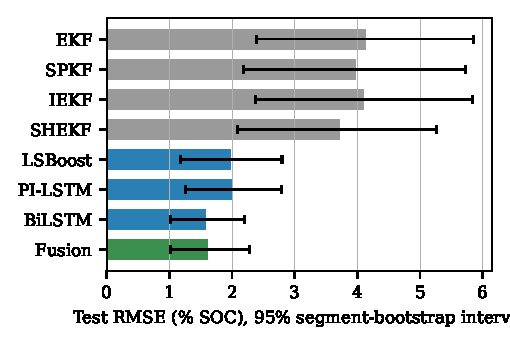
\includegraphics[width=0.85\columnwidth]{figs/v8_lg_rmse_ci.pdf}
\caption{LG-L: test RMSE with 95\% segment-bootstrap intervals (axis from zero).}
\label{fig:rmseci}
\end{figure}

\textbf{By temperature and cycle.} Fig.~\ref{fig:pertemp} shows where the gain comes from. At $+10$~$^\circ$C and above every estimator is within about 1.2\% and at $+25$ and $+40$~$^\circ$C the BiLSTM roughly halves the SPKF error (0.48\% against 1.17\% at $+40$~$^\circ$C). Below $0$~$^\circ$C the filters degrade (SPKF 4.53\% at $-10$ and 10.10\% at $-20$~$^\circ$C) and the BiLSTM reaches 2.56\% and 3.09\%, so most of the absolute gain is in the cold. By cycle (Table~\ref{tab:percycle}) the gain is smallest on US06, where the BiLSTM (2.90\%) is a little better than the SPKF (3.32\%) and LSBoost and the PI-LSTM (4.02\% and 3.97\%) are worse than it. On UDDS and LA92 the BiLSTM is about 74\% below the SPKF, and on HWFET the learners (2.63--3.21\%) are far below the SPKF (6.48\%).

\begin{figure}[!t]
\centering
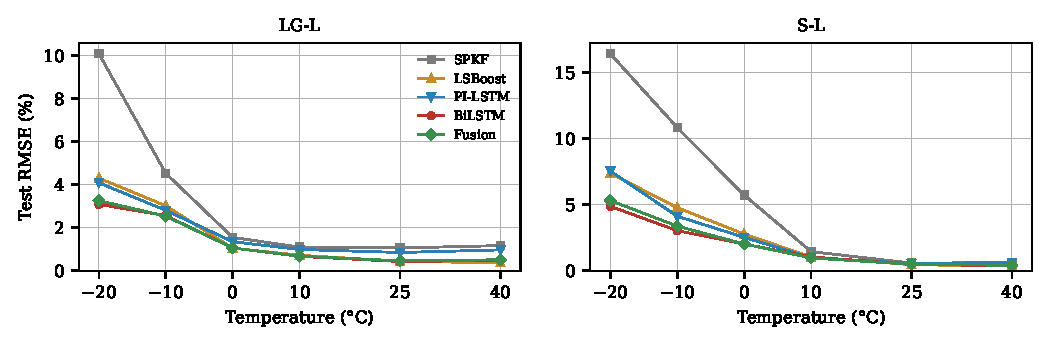
\includegraphics[width=\columnwidth]{figs/v8_pertemp_loco.pdf}
\caption{Test RMSE by chamber temperature, LG-L (left) and S-L (right). The axes start at zero.}
\label{fig:pertemp}
\end{figure}

\begin{table}[!t]
\caption{LG-L: Test RMSE (\%) by Drive Cycle (SPKF Prior)}
\label{tab:percycle}
\centering\footnotesize
\begin{tabular}{@{}lcccccc@{}}
\toprule
Cycle & EKF & SPKF & LSBoost & PI-LSTM & BiLSTM & Fusion\\
\midrule
UDDS & 3.53 & 3.42 & 1.24 & 1.09 & 0.88 & 0.84 \\
HWFET & 6.53 & 6.48 & 2.70 & 3.21 & 2.63 & 2.99 \\
LA92 & 3.62 & 3.48 & 1.06 & 0.88 & 0.88 & 0.90 \\
US06 & 3.93 & 3.32 & 4.02 & 3.97 & 2.90 & 2.72 \\
\bottomrule

\end{tabular}
\end{table}

% Fig.~tracking moved to the supplementary PDF (TTE length).
\noindent\textit{Supplementary Fig.~S1} shows LG-L SOC tracking on UDDS at $25$~$^\circ$C and $-20$~$^\circ$C from a wrong initial SOC: at $-20$~$^\circ$C the filters keep an offset for the whole record.

\subsection{Start-Up, Coulomb Counting, and Convergence}\label{sec:checks}
Every estimator starts with a 10--20\% SOC error. Table~\ref{tab:cc} separates what the estimators add to Coulomb counting. With the true initial SOC and capacity, Coulomb counting reaches 0.07\% RMSE on LG-L, which no estimator here matches; with the wrong initial SOC alone it stays at 14.50\%, and with a 0.08~A current offset and a 1\% gain error in addition at 18.45\%, because it cannot correct the initial error. The estimators therefore earn their place only when the initial SOC is unknown. Convergence into $\pm2$\% (Supplementary Table~S1) takes a median of about 100~s for the EKF and SHEKF on LG-L and converges in 86--91\% of the segments; the learners and the SPKF reach the 30~s minimum set by the window length, and the LSTM+KF does the same. At the cold temperatures of the extrapolation protocols convergence is much slower for every estimator: on LG-E the median is 824--2050~s for the filters and 1705--1995~s for the learners, and on S-E only 25--50\% of segments converge.

\begin{table}[!t]
\caption{Coulomb Counting With and Without Knowledge of the Initial SOC: RMSE and Maximum Error (\%)}
\label{tab:cc}
\centering\scriptsize
\setlength{\tabcolsep}{3pt}
\begin{tabular}{@{}lcccc@{}}
\toprule
 & \multicolumn{2}{c}{LG-L} & \multicolumn{2}{c}{S-L}\\
Variant & RMSE & Max & RMSE & Max\\
\midrule
CC, ideal & 0.072 & 0.35 & 0.088 & 0.42 \\
CC, initial SOC error only & 14.504 & 23.61 & 14.899 & 19.62 \\
CC, realistic & 18.445 & 28.80 & 16.669 & 22.58 \\
\bottomrule

\end{tabular}
\end{table}

\textbf{SPKF diagnostic.} The minimum eigenvalue of $\mP$ stayed positive for every filter on every segment, and no Cholesky factorisation failed with either sigma-point scaling (Supplementary Table~S2). The divergence episodes that led to an earlier choice of the SHEKF prior are therefore not a loss of positive definiteness of $\mP$; they come from the initial error and the cold temperatures.

\subsection{What Carries the Gain}
Table~\ref{tab:component} isolates the components with the selected prior (SPKF on both Kollmeyer cells). Removing the Kalman priors from the BiLSTM input raises its RMSE from 1.57\% to 3.00\% (LG) and from 2.24\% to 2.80\% (Samsung), and that of LSBoost from 1.97\% to 4.75\% and from 3.34\% to 4.33\%. Giving the BiLSTM the priors as inputs only, without the residual target, is also worse (2.71\% LG, 3.78\% Samsung). The priors are not always helpful: on B-W a BiLSTM without priors reaches 1.74\% against 3.49\% with them (Section~\ref{sec:braun}), and on S-E the BiLSTM with priors as inputs only (8.28\%) is slightly better than the residual version (8.50\%).

\begin{table}[!t]
\caption{Component Ablations, Selected Prior (SPKF) (Test RMSE, \%; Last Column: Change Versus the Ablated Variant)}
\label{tab:component}
\centering\scriptsize
\setlength{\tabcolsep}{2pt}
\begin{tabular}{@{}p{3.9cm}ccc@{}}
\toprule
\multicolumn{4}{@{}l}{LG-L}\\
Ablated variant & RMSE & Full & Gain\\
\midrule
PI-LSTM without physics residual ($\lambda=0$) & 1.986 & 1.992 & -0.3\% \\
BiLSTM without Kalman priors & 2.995 & 1.573 & 47.5\% \\
BiLSTM, priors as inputs only (no residual target) & 2.705 & 1.573 & 41.9\% \\
LSBoost without Kalman priors & 4.752 & 1.969 & 58.6\% \\
LSBoost, priors as inputs only (no residual target) & 2.192 & 1.969 & 10.1\% \\
\midrule
\multicolumn{4}{@{}l}{S-L}\\
\bottomrule

PI-LSTM without physics residual ($\lambda=0$) & 3.264 & 3.154 & 3.4\% \\
BiLSTM without Kalman priors & 2.796 & 2.244 & 19.7\% \\
BiLSTM, priors as inputs only (no residual target) & 3.776 & 2.244 & 40.6\% \\
LSBoost without Kalman priors & 4.325 & 3.343 & 22.7\% \\
LSBoost, priors as inputs only (no residual target) & 3.505 & 3.343 & 4.6\% \\
\bottomrule

\end{tabular}
\end{table}

\textbf{The Coulomb-counting loss.} Over five seeds the PI-LSTM with and without the physics term is $2.003\pm0.014$ and $1.994\pm0.016$ on LG-L, $3.230\pm0.132$ and $3.455\pm0.122$ on S-L, $2.236\pm0.166$ and $2.456\pm0.154$ on B-W, and $1.643\pm0.112$ and $1.694\pm0.116$ on B-R (mean $\pm$ standard deviation, \%; selected prior, except B-R, where the SPKF-prior run has one seed without the term, so the SHEKF-prior pair is shown). Across the nine protocols with five seeds on both sides the term lowers the mean RMSE in seven and raises it in LG-L (by 0.01 points) and S-S (by 0.06). The largest gains are on S-L (0.23 points, 1.7 seed standard deviations), B-W (0.22, 1.3), and LG-T (0.15, 1.3). With nine comparisons and five seeds we cannot separate these from seed noise and do not claim a benefit of the term. The PI-LSTM's value is its architecture: it adds its correction to the Kalman trajectory and is the estimator that stays accurate under the regime shift of B-R.

\textbf{Fusion rules.} On LG-L the simplex NNLS (1.61\%) beats equal weights (2.65\%) and inverse-MSE weights (2.00\%), is close to the unconstrained least squares (1.71\%, with weights down to $-0.40$), cross-fitted and gated variants (1.61--1.68\%), and is not better than simply choosing the best single estimator on validation (1.57\%). On S-L the unconstrained stack (2.54\%) is no better than the simplex (2.42\%), and its weights reach $-3.9$. The weights are sparse (87\% BiLSTM on LG-L and 89\% on S-L, the rest on SHEKF), the PI-LSTM and LSBoost can be removed without change, and removing the BiLSTM raises the LG-L fusion to 1.91\%. A stack of the learners alone is as good as the full stack (LG-L 1.58\% against 1.61\%; S-L 2.24\% against 2.42\%). The stacking layer guarantees a bounded combination; it does not improve on its best member.

\subsection{Second Cell and Zero-Shot Transfer}
On S-L the learners reach 2.24--3.34\% against 6.70\% for the best filter, a reduction of 67\% for the BiLSTM. The LSTM+KF reference reaches 2.07\%, better than the BiLSTM, and the LSTM 2.30\%, level with it. The fusion (2.42\%) is again behind its main member. At $-20$~$^\circ$C the SPKF is at 16.44\% and the BiLSTM at 4.88\%.

\textbf{Zero-shot transfer (S-X).} The LG-trained learners and stacking weights, with no refit, are applied to the Samsung cell, whose filters use Samsung circuit parameters (a calibration of the physical model, not retraining of the learners). The BiLSTM reaches 4.08\% and the fusion 4.35\%, against 6.70\% for the best filter, reductions of 39\% and 35\%. Models trained on the Samsung cell reach 2.44\% (SHEKF prior), so transfer recovers about 61\% of the gain. S-X was run with the SHEKF prior only. Raw-input networks trained on the Samsung cell (fit on its Mixed cycles, tested on the same blocks) reach 2.21--2.94\%, and the LSTM+KF 1.87\%; they use target-cell training data that our transferred learners do not, so this is a reference for what training on the target cell buys, not a like-for-like contest.

\subsection{Held-Out Drive Cycle (LG-C)}
In LG-C the US06 cycle is withheld; the learners are trained on UDDS and HWFET at all temperatures and validated on LA92 (the Mixed files are not used). Table~\ref{tab:lcyc} shows that the best filter, the SPKF (4.95\%), beats every learner (BiLSTM 6.44\%, PI-LSTM 6.95\%, LSBoost 7.50\%) and the fusion (6.21\%), with the lowest maximum error (13.2\% against 18--27\%). The learners remain better than the raw-input references (7.30--11.44\%). The result limits the claim of Section~\ref{sec:results}: when a drive cycle is far from the training cycles and training data are few, the learned correction does not carry over, and with the SPKF prior the BiLSTM (5.34\%) is closer to the filter than with the SHEKF prior chosen by the validation rule (6.44\%). We have not tried to repair this.

\begin{table}[!t]
\caption{LG-C: Test RMSE (\%) on the Held-Out US06 Cycle (Filters Do Not Depend on the Prior; Learners Shown for the SPKF and the SHEKF Prior)}
\label{tab:lcyc}
\centering\scriptsize
\begin{tabular}{@{}lcc@{}}
\toprule
Estimator & SPKF prior & SHEKF prior\\
\midrule
EKF & \multicolumn{2}{c}{6.66} \\
SPKF & \multicolumn{2}{c}{4.95} \\
IEKF & \multicolumn{2}{c}{6.61} \\
SHEKF & \multicolumn{2}{c}{5.78} \\
\midrule
LSBoost & 7.41 & 7.50 \\
PI-LSTM & 6.68 & 6.95 \\
BiLSTM & 5.34 & 6.44 \\
Fusion & 5.93 & 6.21 \\
LSTM & \multicolumn{2}{c}{7.93} \\
GRU & \multicolumn{2}{c}{11.44} \\
CNN-LSTM & \multicolumn{2}{c}{8.46} \\
LSTM+KF & \multicolumn{2}{c}{7.30} \\
\bottomrule

\end{tabular}
\end{table}

\subsection{Temperature Generalisation}\label{sec:temp}
\textbf{Effect of the Arrhenius model.} Table~\ref{tab:ecmabl} repeats the six temperature protocols with the nearest-temperature parameter lookup and with the Arrhenius model (SHEKF prior; both use five seeds). At the held-out $0$~$^\circ$C on LG the best filter improves from 4.36\% to 2.04\% and the BiLSTM from 2.93\% to 1.49\%. In extrapolation the best filter goes from 10.58\% to 6.05\% and the BiLSTM from 9.39\% to 6.65\%. On the Samsung cell the gain is smaller for the filters (3\% in S-T, 18\% in S-E) and larger for the learners (10\% and 23\%). Under sparse calibration the Arrhenius model makes the best filter worse (LG-S 3.67\% to 4.58\%, S-S 5.46\% to 6.05\%) and gives the learners a gain of 4.5\% and 15.5\%. A line in $1/T$ through three points, one of them at $-20$~$^\circ$C, is dominated by the coldest point, which would explain it; we did not test that explanation.

\begin{table}[!t]
\caption{Nearest-Temperature Lookup (N) Versus Arrhenius Model (A), SHEKF Prior: Test RMSE (\%) and Change}
\label{tab:ecmabl}
\centering\scriptsize
\setlength{\tabcolsep}{2.2pt}
\begin{tabular}{@{}lccccccccc@{}}
\toprule
 & \multicolumn{3}{c}{Best filter} & \multicolumn{3}{c}{BiLSTM} & \multicolumn{3}{c}{Fusion}\\
 & N & A & Chg. & N & A & Chg. & N & A & Chg.\\
\midrule
LG-T & 4.36 & 2.04 & -53\% & 2.93 & 1.49 & -49\% & 3.01 & 1.46 & -52\% \\
S-T & 5.89 & 5.69 & -3\% & 1.74 & 1.56 & -10\% & 2.10 & 1.81 & -14\% \\
LG-E & 10.58 & 6.05 & -43\% & 9.39 & 6.65 & -29\% & 9.73 & 6.59 & -32\% \\
S-E & 12.99 & 10.68 & -18\% & 10.34 & 7.99 & -23\% & 12.69 & 9.64 & -24\% \\
LG-S & 3.67 & 4.58 & +25\% & 4.09 & 3.90 & -4\% & 3.93 & 3.89 & -1\% \\
S-S & 5.46 & 6.05 & +11\% & 2.35 & 1.99 & -15\% & 2.62 & 2.38 & -9\% \\
\bottomrule

\end{tabular}
\end{table}

\textbf{What the extrapolation gets wrong.} The parameter oracle (Supplementary Table~S3) replaces one extrapolated quantity at a time by its directly identified value. On LG at $0$~$^\circ$C the resistance is the main cause: with $R_0$ identified directly the EKF error falls from 2.78 to 2.13\%, and with all parameters direct to 1.81\%. At $-10$~$^\circ$C direct $R_0$ lowers it from 5.11 to 4.56\%. At $-20$~$^\circ$C replacing the parameters changes little (EKF 10.62\% extrapolated, 10.31\% with all parameters direct; direct $R_0$ alone makes it worse, 13.45\%). The error at $-20$~$^\circ$C on LG is therefore not caused by the extrapolated parameters; it is a limit of the one-branch model and its OCV table in the cold, which parameter identification cannot repair. On the Samsung cell the parameters matter more but do not close the gap: at $-20$~$^\circ$C the EKF falls from 17.49\% to 13.90\% with $R_0$, $R_1$, and $\tau_1$ direct, still more than three times the warm-temperature error. A constant $\tau_1$ (the median of the identified ones) is no worse than the Arrhenius $\tau_1$ and better at $0$~$^\circ$C (EKF 2.41\% against 2.78\%), so the Arrhenius law for $\tau_1$ is not supported; the part of the model that is supported is the law for $R_0$.

\textbf{Held-out temperature and sparse calibration.} With $0$~$^\circ$C never seen, the BiLSTM (1.58\%) and fusion (1.59\%) beat the best filter (2.04\%) by 23\%, and the LSTM+KF reference is level with them (1.69\% in this run and 1.24\% in the retraining that accompanied the SHEKF prior, so neither ranking is secure). LSBoost fails at this temperature (5.59\%) and still receives validation weight. On the Samsung cell the learners clearly separate from the filters: BiLSTM 1.50\% against 5.69\% for the best filter. With the circuit identified at only $40$, $10$, and $-20$~$^\circ$C, the BiLSTM reaches 3.09\% on LG against 4.58\% for the best filter, and the PI-LSTM 2.13\% on Samsung against 6.05\%.

\textbf{Extrapolation (LG-E, S-E).} Training at $+10$ to $+40$~$^\circ$C and testing at $0$, $-10$, and $-20$~$^\circ$C (Fig.~\ref{fig:tempx}, Table~\ref{tab:tempxpt}). On LG every estimator sits between 6.05 and 6.78\%: the learners do not improve on the filters, and the error at $-20$~$^\circ$C is 10.30--10.94\% for all of them. The raw-input models do not survive: LSTM 19.62\%, GRU 15.00\%, CNN-LSTM 12.09\%, LSTM+KF 16.63\%. On Samsung the situation differs: the BiLSTM is the best of ours (8.50\%) against 10.68\% for the best filter, but the LSTM+KF (7.29\%) and the LSTM (7.75\%) are better, and only GRU and CNN-LSTM (11.03--12.42\%) are worse. The Kalman prior therefore protects against the failure of raw-input networks on the LG cell and not on the Samsung cell. At $-20$~$^\circ$C the best of our estimators reaches 10.30\% on LG and 13.36\% on Samsung, which we report as the principal limitation.

\begin{figure}[!t]
\centering
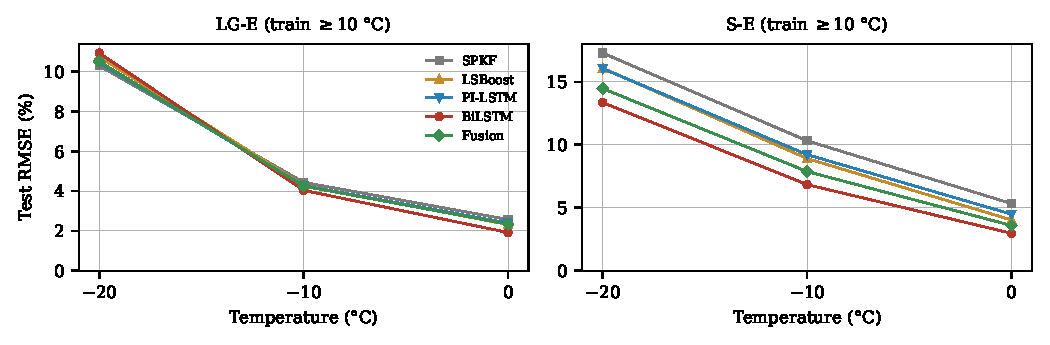
\includegraphics[width=\columnwidth]{figs/v8_pertemp_tempx.pdf}
\caption{Extrapolation: test RMSE versus temperature when training uses only $\ge10$~$^\circ$C (SPKF prior, Arrhenius parameters). The axes start at zero.}
\label{fig:tempx}
\end{figure}

\begin{table}[!t]
\caption{LG-E and S-E: Test RMSE (\%) by Temperature (SPKF, LSBoost, PI-LSTM, BiLSTM, Fusion; SPKF Prior)}
\label{tab:tempxpt}
\centering\scriptsize
\setlength{\tabcolsep}{2.4pt}
\begin{tabular}{@{}rccccc@{\hspace{6pt}}ccccc@{}}
\toprule
 & \multicolumn{5}{c}{LG-E} & \multicolumn{5}{c}{S-E}\\
$T$ & SPKF & LSB. & PI & BiL. & Fus. & SPKF & LSB. & PI & BiL. & Fus.\\
\midrule
$0$ & 2.57 & 2.32 & 2.40 & 1.92 & 2.34 & 5.33 & 4.03 & 4.49 & 2.97 & 3.59 \\
$-10$ & 4.44 & 4.29 & 4.27 & 4.04 & 4.25 & 10.32 & 8.91 & 9.22 & 6.84 & 7.88 \\
$-20$ & 10.30 & 10.75 & 10.45 & 10.94 & 10.51 & 17.29 & 16.09 & 16.04 & 13.36 & 14.47 \\
\bottomrule

\end{tabular}
\end{table}

\subsection{Long WLTP Record (Braun)}\label{sec:braun}
All four filters have an RMSE floor of about 3.7--4.3\% on this record. On B-W (training includes the first 30\% of the WLTP block) the PI-LSTM reaches 2.29\% and the fusion 2.39\% against 4.14\% for the filters, but GRU (1.94\%) and LSTM+KF (2.25\%) are better, the LSTM (2.39\%) is level, and a BiLSTM without priors reaches 1.74\%. On B-R (training on constant-current cycling only) the PI-LSTM reaches 1.30\%, while the BiLSTM, LSBoost, and fusion do little or nothing against the filters (3.74, 5.08, and 3.44\% against 3.74\%), and the raw-input references fail (8.42--12.10\% for CNN-LSTM, GRU, LSTM, and LSTM+KF). The BiLSTM is also the least stable network across seeds on B-R ($\pm$1.0 points).

The reference needs a caution. The Braun SOC is Coulomb counted at 19.96~Ah, and the filter floor drifts slowly over the 21~h block. Adding a $+0.67$~A current offset to the test current lowers the filter RMSE from 4.14\% to 1.49\% on B-W, which is a sign that the label, not the voltage model, carries part of the error. The PI-LSTM may therefore partly learn the behaviour of the label. On the aged cell, with nothing refitted, the filters keep an error of 1.7\% while the PI-LSTM and the fusion degrade to 4.08\% and 4.07\% (Supplementary Table~S4). We read the Braun results as evidence that the PI-LSTM architecture can cross a regime shift on one cell, not as evidence of better SOC accuracy than the filters on an aged cell. The record has three segments, so the intervals use 30-minute units and are wide.

\subsection{Robustness and Uncertainty}
Table~\ref{tab:robust} perturbs the LG-L test segments with the trained models fixed (SPKF prior). A further 15-point initial SOC error leaves the BiLSTM at 1.57\% and raises the fusion from 1.61\% to 1.66\%; the filters are unchanged (their start-up error is already present). Noise of 10~mV and 0.082~A, a $+2$\% current gain error, and a current offset change the learners by at most about 0.11 points. The fusion is not worse than the SPKF in any scenario on either Kollmeyer cell. With the SHEKF prior the same perturbations move the BiLSTM by up to 0.14 points (1.69\% to 1.83\% for the extra start-up error).

\begin{table}[!t]
\caption{LG-L Robustness: Test RMSE (\%) Under Perturbed Test Inputs (SPKF Prior)}
\label{tab:robust}
\centering\scriptsize
\setlength{\tabcolsep}{2.2pt}
\begin{tabular}{@{}p{2.55cm}cccccc@{}}
\toprule
Scenario & EKF & SPKF & LSB. & PI & BiL. & Fus.\\
\midrule
Nominal (default start-up error) & 4.12 & 3.97 & 1.97 & 1.99 & 1.57 & 1.61 \\
Extra initial SOC shift -15 points & 4.12 & 4.00 & 1.97 & 2.05 & 1.57 & 1.66 \\
Noise 10 mV and 0.082 A & 4.11 & 3.98 & 1.98 & 2.00 & 1.57 & 1.60 \\
Current offset +0.082 A & 3.94 & 3.79 & 2.08 & 2.03 & 1.63 & 1.58 \\
Current gain error +2 percent & 4.08 & 3.90 & 1.99 & 2.00 & 1.57 & 1.59 \\
\bottomrule

\end{tabular}
\end{table}

\textbf{Conformal intervals.} A split-conformal interval~\cite{lei2018conformal,vovk2005algorithmic} with 90\% target coverage reaches 90.8\% on the LG-L test block (width 4.96\% SOC) and 88.0\% on S-L (6.36\%), but not uniformly over temperature: on LG-L coverage is 99.8\% or more at $+10$~$^\circ$C and warmer and falls to 74.0\% at $-10$ and 64.6\% at $-20$~$^\circ$C, and a temperature-conditional interval has 90.9\% coverage at a width of 4.91\%. Under shift the guarantee breaks, as expected for intervals that rest on exchangeability: coverage is 92.1\% on LG-T (close to the target), 52.9\% on LG-E, 8.1\% on S-E, 9.4\% on B-W, and 0.6\% on B-R. The intervals are reported only for the in-distribution protocols.

\subsection{Latency and Deployment}\label{sec:latency}
In MATLAB on one CPU thread a single estimate costs 0.02--0.05~ms for each filter, 1.1--3.2~ms for the recurrent networks, 15~ms for LSBoost, and 16--20~ms for the full stack (Table~\ref{tab:main}); LSBoost dominates the stack. To check that the cost is compatible with embedded hardware, the arithmetic of the networks was timed on an Arduino UNO Q (an aarch64 Linux board) with a NumPy float32 implementation on one thread (Table~\ref{tab:edge}). With random weights matching the trained layer sizes, a BiLSTM estimate takes about 22~ms, a PI-LSTM estimate 11~ms, and the timed stack of SHEKF, BiLSTM, and PI-LSTM about 33~ms (two runs; 99th percentile 34--36~ms, worst case 42~ms), with a peak resident memory of 34.6~MB. Timing with the exported trained weights on the same board raised the BiLSTM median to about 36~ms and the stack to about 54~ms (two runs; peak RSS 35~MB); the board still establishes cost, not accuracy. Even the slower trained-weight stack is under 6\% of the one-second sampling period. The 30-sample window is recomputed at every second in this implementation; compiled code and streaming evaluation of the unidirectional PI-LSTM would be cheaper. Table~\ref{tab:edge} also lists the parameter and multiply-accumulate counts, which follow from the layer sizes. These numbers are for a development board and do not establish performance on an automotive controller.

\begin{table}[!t]
\caption{Cost per Estimate (30-Sample Window, fp32). Parameters and MACs are Analytic; Times are Medians Measured on an Arduino UNO Q in Two Runs}
\label{tab:edge}
\centering\scriptsize
\setlength{\tabcolsep}{2.4pt}
\begin{tabular}{@{}lcccc@{}}
\toprule
Estimator & Params & MACs & MB & UNO Q (ms)\\
\midrule
EKF/IEKF/SHEKF & -- & $<10^{3}$ & -- & 0.21/0.47/0.24\\
SPKF & -- & $<10^{3}$ & -- & 0.97 / 0.87\\
BiLSTM & 158\,849 & $4.20\times10^{6}$ & 0.64 & 22.2 / 21.4\\
PI-LSTM & 75\,841 & $2.14\times10^{6}$ & 0.30 & 11.0 / 10.9\\
SHEKF+BiLSTM+PI-LSTM & 234\,690 & $6.34\times10^{6}$ & 0.94 & 33.6 / 32.8\\
\bottomrule
\end{tabular}
\end{table}

\section{What Did Not Help}\label{sec:neg}
The negative and neutral results, collected in one place because they bound the claims of the paper.
\begin{itemize}
\item \textbf{Stacking.} The simplex stack is not the most accurate estimator in any protocol. A stack of the learners alone, or the best single estimator on validation, is as good (Table~\ref{tab:prior} and Section~\ref{sec:results}). Its guarantee is a bounded combination, not a better one.
\item \textbf{The Coulomb-counting loss.} No benefit beyond seed noise on any protocol.
\item \textbf{Unconstrained least squares.} Equal or worse than the simplex stack on both cells, with weights as low as $-3.9$.
\item \textbf{The SHEKF as a default prior.} The SPKF prior has the lower validation error in nine of eleven protocols; the SPKF did not diverge and its covariance stayed positive definite.
\item \textbf{Learners on a held-out drive cycle.} On LG-C the best filter is better than every learner.
\item \textbf{Learners against the filters in extrapolation on LG.} On LG-E the learners are level with the best filter.
\item \textbf{LSBoost under shift.} It fails at the held-out temperature of the LG cell and still receives validation weight.
\item \textbf{Conformal intervals under shift.} Coverage of the 90\% target is 53\% on LG-E, 8\% on S-E, and below 10\% on the Braun protocols.
\item \textbf{The Arrhenius law for $\tau_1$ and for sparse calibration.} A constant $\tau_1$ is no worse; under sparse calibration the filters are worse than with a nearest lookup.
\item \textbf{Parameter identification at $-20$~$^\circ$C.} Direct identification of the circuit parameters does not remove the cold-temperature error on LG.
\item \textbf{Raw-input hybrids.} An LSTM fused with Coulomb counting, and on B-W a GRU, is more accurate than our estimators on four protocols.
\item \textbf{Aged-cell transfer.} On the Braun record the filters keep their error and the learners degrade.
\end{itemize}

\section{Scope and Limitations}
The evidence supports the following scope. In range, a BiLSTM that corrects a Kalman prior is clearly better than the filters on the Kollmeyer cells (by 58--67\% on unseen cycles), the Arrhenius circuit model makes filters usable at a temperature with no identification data, and the learners transfer to a second cell with the circuit recalibrated. The evidence does not support the following: accuracy at $-20$~$^\circ$C without training data there; a benefit of the stacking layer, of the physics term, or of the Arrhenius law for the time constant; generalisation to a drive cycle far from the training cycles with little training data (LG-C); superiority over a raw-input LSTM fused with Coulomb counting in range; or protection by the prior against failure outside the training range on every cell (it holds for LG and not for Samsung).

The design of the study sets further limits. Every estimator starts from a 10--20\% initial error, which lifts the filter errors; results with the true initial SOC would differ, and Coulomb counting is then very accurate (Table~\ref{tab:cc}). The prior is chosen on a validation block that, for LG-E and S-E, lies inside the training temperature range, so the choice there says little about extrapolation. Seeds, ablations, robustness, and conformal intervals use the selected prior of each protocol; the raw-input references were run on ten of the eleven protocols and, on LG-T, differ by 0.4 points between two retrainings; the Braun record has three segments. Reference SOC on the Kollmeyer cells is derived from the cycler's Ah counter and the capacity at 95\% discharge, and a bias in it would be shared by filters and learners; the Braun reference has a known inconsistency with the voltage. The Kollmeyer records contain discharge profiles repeated to 95\% discharge, so full charge--discharge cycling is not covered, and no LFP cell is included. Only Mixed1 to Mixed3 remain at $+40$~$^\circ$C after cleaning, so the $+40$~$^\circ$C fit and validation blocks are small. Parameters are identified offline, ageing of the Kollmeyer cells was not studied, and the identified $R_1$ at $-10$ and $-20$~$^\circ$C is nearly equal (64.54 and 64.50~m$\Omega$, all eight multi-starts agreeing at each temperature, so a flat optimum of the voltage fit and not a bound; $R_0$ and $\tau_1$ still differ). The embedded measurement uses random weights and a development board. The comparisons with published methods are with our implementations of their ideas on our splits. Future work includes an online parameter update, a cold-temperature term beyond the one-branch model, regime-dependent weights, training that includes the start-up error, deployment of the trained models on the board, and aged-cell data.

\section{Conclusion}
This paper asked whether Kalman-filter estimates can carry a learned SOC estimator across cycles, temperatures, and cells, and where they cannot. In range they can. With a Kalman prior and a residual target, a BiLSTM lowers the error of the best filter by 58\% on unseen cycles of the LG cell and by 67\% on the Samsung cell, from a 10--20\% start-up error, and the gain is largest in the cold. An Arrhenius circuit model lets the filters run at unmeasured temperatures and lowers the best-filter error by 53\% at a held-out temperature and by 43\% in extrapolation; the resistance law is the useful part, and it does not help under sparse calibration.

The limits are as clear. Outside the training temperature range the prior keeps the LG learners bounded where raw-input networks fail, but on the Samsung cell raw-input networks are as good, and at $-20$~$^\circ$C no method is accurate (about 10.30\% on LG, 13.36\% on Samsung) even with directly identified parameters. On a held-out drive cycle with little training data the best filter beats every learner. The stacking layer and the physics term do not improve the accuracy.

For practice we draw three conclusions. A filter with the Arrhenius resistance law is a safe baseline at any temperature of use. A prior-based BiLSTM is worth adding where training data cover the temperature range and the drive cycles. Calibration or training data at the coldest temperature of use cannot be replaced by any of the methods tested here.

\section*{Acknowledgment}
Data from Kollmeyer \emph{et al.} (LG 18650HG2 and Samsung INR21700-30T) and from Braun \emph{et al.} (CC BY-NC 4.0) are gratefully acknowledged. AI assistance (Claude, Anthropic) was used for code development, drafting, and editing; the authors reviewed all content and take responsibility for it.

\section*{Data and Code Availability}
The three datasets are public (doi:10.17632/b5mj79w5w9.2, doi:10.17632/9xyvy2njj3.2, doi:10.5281/zenodo.6985321). The MATLAB pipeline, the batch runner, the result tables for every protocol, and the embedded benchmark script are available from the corresponding author on request and will be deposited in a public repository on acceptance.

\begin{thebibliography}{99}
\bibitem{xiong2018review} R.~Xiong, J.~Cao, Q.~Yu, H.~He, and F.~Sun, ``Critical review on the battery state of charge estimation methods for electric vehicles,'' \emph{IEEE Access}, vol.~6, pp. 1832--1843, 2018.
\bibitem{plett2015bms} G.~L. Plett, \emph{Battery Management Systems, Volume I: Battery Modeling}. Norwood, MA, USA: Artech House, 2015.
\bibitem{plett2004ekf} G.~L. Plett, ``Extended Kalman filtering for battery management systems of LiPB-based HEV battery packs: Part 3. State and parameter estimation,'' \emph{J. Power Sources}, vol.~134, no.~2, pp. 277--292, Aug. 2004.
\bibitem{chen2013ekf} Z.~Chen, Y.~Fu, and C.~C. Mi, ``State of charge estimation of lithium-ion batteries in electric drive vehicles using extended Kalman filtering,'' \emph{IEEE Trans. Veh. Technol.}, vol.~62, no.~3, pp. 1020--1030, Mar. 2013.
\bibitem{chemali2017lstm} E.~Chemali, P.~J. Kollmeyer, M.~Preindl, R.~Ahmed, and A.~Emadi, ``Long short-term memory networks for accurate state-of-charge estimation of Li-ion batteries,'' \emph{IEEE Trans. Ind. Electron.}, vol.~65, no.~8, pp. 6730--6739, Aug. 2018.
\bibitem{plett2006spkf} G.~L. Plett, ``Sigma-point Kalman filtering for battery management systems of LiPB-based HEV battery packs: Part 2. Simultaneous state and parameter estimation,'' \emph{J. Power Sources}, vol.~161, no.~2, pp. 1369--1384, Oct. 2006.
\bibitem{julier2004ukf} S.~J. Julier and J.~K. Uhlmann, ``Unscented filtering and nonlinear estimation,'' \emph{Proc. IEEE}, vol.~92, no.~3, pp. 401--422, Mar. 2004.
\bibitem{bell1993iekf} B.~M. Bell and F.~W. Cathey, ``The iterated Kalman filter update as a Gauss-Newton method,'' \emph{IEEE Trans. Autom. Control}, vol.~38, no.~2, pp. 294--297, Feb. 1993.
\bibitem{sage1969adaptive} A.~P. Sage and G.~W. Husa, ``Adaptive filtering with unknown prior statistics,'' in \emph{Proc. Joint Autom. Control Conf.}, Boulder, CO, USA, 1969, pp. 760--769.
\bibitem{xiong2013aekf} R.~Xiong, H.~He, F.~Sun, and K.~Zhao, ``Evaluation on state of charge estimation of batteries with adaptive extended Kalman filter by experiment approach,'' \emph{IEEE Trans. Veh. Technol.}, vol.~62, no.~1, pp. 108--117, Jan. 2013.
\bibitem{breiman1996stacked} L.~Breiman, ``Stacked regressions,'' \emph{Mach. Learn.}, vol.~24, no.~1, pp. 49--64, Jul. 1996.
\bibitem{lawson1974lsq} C.~L. Lawson and R.~J. Hanson, \emph{Solving Least Squares Problems}. Englewood Cliffs, NJ, USA: Prentice-Hall, 1974.
\bibitem{krogh1995ensembles} A.~Krogh and J.~Vedelsby, ``Neural network ensembles, cross validation, and active learning,'' in \emph{Advances in Neural Information Processing Systems 7}, 1995, pp. 231--238.
\bibitem{beck2009fista} A.~Beck and M.~Teboulle, ``A fast iterative shrinkage-thresholding algorithm for linear inverse problems,'' \emph{SIAM J. Imaging Sci.}, vol.~2, no.~1, pp. 183--202, 2009.
\bibitem{duchi2008simplex} J.~Duchi, S.~Shalev-Shwartz, Y.~Singer, and T.~Chandra, ``Efficient projections onto the $\ell_1$-ball for learning in high dimensions,'' in \emph{Proc. 25th Int. Conf. Mach. Learn.}, 2008, pp. 272--279, doi:10.1145/1390156.1390191.
\bibitem{lei2018conformal} J.~Lei, M.~G'Sell, A.~Rinaldo, R.~J. Tibshirani, and L.~Wasserman, ``Distribution-free predictive inference for regression,'' \emph{J. Amer. Statist. Assoc.}, vol.~113, no.~523, pp. 1094--1111, 2018, doi:10.1080/01621459.2017.1307116.
\bibitem{vovk2005algorithmic} V.~Vovk, A.~Gammerman, and G.~Shafer, \emph{Algorithmic Learning in a Random World}. New York, NY, USA: Springer, 2005.
\bibitem{hannan2017review} M.~A. Hannan, M.~S.~H. Lipu, A.~Hussain, and A.~Mohamed, ``A review of lithium-ion battery state of charge estimation and management system in electric vehicle applications: Challenges and recommendations,'' \emph{Renew. Sustain. Energy Rev.}, vol.~78, pp. 834--854, Oct. 2017.
\bibitem{zhao2024wevj} F.~Zhao, Y.~Guo, and B.~Chen, ``A review of lithium-ion battery state of charge estimation methods based on machine learning,'' \emph{World Electr. Veh. J.}, vol.~15, no.~4, Art.~131, 2024.
\bibitem{hu2026ionics} J.~Hu, X.~Wang, Z.~Wang, and K.~Deng, ``The state-of-the-art in state of charge estimation methods for lithium-ion batteries: Ongoing evolution and future perspective,'' \emph{Ionics}, vol.~32, no.~8, pp. 7831--7862, 2026.
\bibitem{wang2025rser} Y.~Wang \emph{et al.}, ``A comprehensive review of machine learning-based state of health estimation for lithium-ion batteries: Data, features, algorithms, and future challenges,'' \emph{Renew. Sustain. Energy Rev.}, vol.~224, Art.~116125, 2025.
\bibitem{xu2025processes} H.~Xu, F.~Zhao, and Y.~Guo, ``State of charge estimation for lithium-ion batteries: An online method combining deep neural network and adaptive Kalman filter,'' \emph{Processes}, vol.~13, no.~11, Art.~3559, 2025.
\bibitem{jiang2025energy} H.~Jiang, L.~Yin, Z.~Xu, L.~Hu, W.~Huang, and Y.~Zhao, ``A novel hybrid framework for SOC estimation using PatchMixer-LSTM and adaptive UKF,'' \emph{Energy}, vol.~335, Art.~137891, 2025.
\bibitem{pollo2025date} G.~Pollo, A.~Burrello, E.~Macii, M.~Poncino, S.~Vinco, and D.~Jahier Pagliari, ``Coupling neural networks and physics equations for Li-ion battery state-of-charge prediction,'' in \emph{Proc. Design, Autom. Test Eur. Conf. (DATE)}, 2025, arXiv:2412.16724.
\bibitem{previtali2025iecon} D.~Previtali, D.~Masti, M.~Mazzoleni, and F.~Previdi, ``A virtual sensor fusion approach for state of charge estimation of lithium-ion cells,'' in \emph{Proc. IEEE Annu. Conf. Ind. Electron. Soc. (IECON)}, 2025, arXiv:2508.04268.
\bibitem{carrera2025sensors} R.~Carrera, L.~Quiroz, C.~Guevara, and P.~Acosta-Vargas, ``State-of-charge estimation of medium- and high-voltage batteries using LSTM neural networks optimized with genetic algorithms,'' \emph{Sensors}, vol.~25, no.~15, Art.~4632, 2025.
\bibitem{braun2022dataset} J.~A. Braun, R.~Behmann, D.~Schmider, and W.~G. Bessler, ``Code and measurement data: State of charge and state of health diagnosis of batteries with voltage-controlled models,'' Zenodo, v1.1, Jul. 2022, doi:10.5281/zenodo.6985321.
\bibitem{kollmeyer2020lg} P.~Kollmeyer, M.~Naguib, and M.~Skells, ``LG 18650HG2 Li-ion battery data,'' Mendeley Data, V2, Jan. 2020, doi:10.17632/b5mj79w5w9.2.
\bibitem{kollmeyer2020samsung} P.~Kollmeyer, ``Samsung INR21700 30T 3Ah Li-ion battery data,'' Mendeley Data, V2, Dec. 2023, doi:10.17632/9xyvy2njj3.2.
\bibitem{hu2012ecm} X.~Hu, S.~Li, and H.~Peng, ``A comparative study of equivalent circuit models for {Li}-ion batteries,'' \emph{J. Power Sources}, vol.~198, pp.~359--367, 2012.
\bibitem{waag2014review} W.~Waag, C.~Fleischer, and D.~U. Sauer, ``Critical review of the methods for monitoring of lithium-ion batteries in electric and hybrid vehicles,'' \emph{J. Power Sources}, vol.~258, pp.~321--339, 2014.
\bibitem{jaguemont2016cold} J.~Jaguemont, L.~Boulon, and Y.~Dub{\'e}, ``A comprehensive review of lithium-ion batteries used in hybrid and electric vehicles at cold temperatures,'' \emph{Appl. Energy}, vol.~164, pp.~99--114, 2016.
\bibitem{vidal2020ffnn} C.~Vidal, P.~Kollmeyer, M.~Naguib, P.~Malysz, O.~Gross, and A.~Emadi, ``Robust {xEV} battery state-of-charge estimator design using a feedforward deep neural network,'' \emph{SAE Tech. Paper} 2020-01-1181, 2020.
\bibitem{vidal2019transfer} C.~Vidal, P.~Kollmeyer, E.~Chemali, and A.~Emadi, ``{Li}-ion battery state of charge estimation using long short-term memory recurrent neural network with transfer learning,'' in \emph{Proc. IEEE Transportation Electrification Conf. Expo (ITEC)}, 2019.
\bibitem{bian2020bilstm} C.~Bian, H.~He, and S.~Yang, ``Stacked bidirectional long short-term memory networks for state-of-charge estimation of lithium-ion batteries,'' \emph{Energy}, vol.~191, p.~116538, 2020.
\bibitem{hochreiter1997lstm} S.~Hochreiter and J.~Schmidhuber, ``Long short-term memory,'' \emph{Neural Comput.}, vol.~9, no.~8, pp.~1735--1780, 1997, doi:10.1162/neco.1997.9.8.1735.
\bibitem{schuster1997birnn} M.~Schuster and K.~K. Paliwal, ``Bidirectional recurrent neural networks,'' \emph{IEEE Trans. Signal Process.}, vol.~45, no.~11, pp.~2673--2681, 1997, doi:10.1109/78.650093.
\bibitem{raissi2019pinn} M.~Raissi, P.~Perdikaris, and G.~E. Karniadakis, ``Physics-informed neural networks: a deep learning framework for solving forward and inverse problems involving nonlinear partial differential equations,'' \emph{J. Comput. Phys.}, vol.~378, pp.~686--707, 2019.
\bibitem{pan2010transfer} S.~J. Pan and Q.~Yang, ``A survey on transfer learning,'' \emph{IEEE Trans. Knowl. Data Eng.}, vol.~22, no.~10, pp.~1345--1359, 2010, doi:10.1109/TKDE.2009.191.
\bibitem{wolpert1992stacked} D.~H. Wolpert, ``Stacked generalization,'' \emph{Neural Netw.}, vol.~5, no.~2, pp.~241--259, 1992, doi:10.1016/S0893-6080(05)80023-1.
\bibitem{friedman2001boost} J.~H. Friedman, ``Greedy function approximation: a gradient boosting machine,'' \emph{Ann. Statist.}, vol.~29, no.~5, pp.~1189--1232, 2001.
\bibitem{kingma2015adam} D.~P. Kingma and J.~Ba, ``Adam: a method for stochastic optimization,'' in \emph{Proc. Int. Conf. Learn. Represent. (ICLR)}, 2015. [Online]. Available: https://arxiv.org/abs/1412.6980
\bibitem{wan2000ukf} E.~A. Wan and R.~van der Merwe, ``The unscented {Kalman} filter for nonlinear estimation,'' in \emph{Proc. IEEE Adaptive Syst. Signal Process., Commun., Control Symp.}, 2000, pp.~153--158, doi:10.1109/ASSPCC.2000.882463.
\end{thebibliography}


\end{document}
